\section{Single variable linear Regression}
\subsection{Notation}
\begin{table}[htb]
	\begin{center}
		\begin{tabular}[h]{ c | l }
			
			\textbf{Notation}    & \textbf{Meaning}\\ \midrule
			m 			 			 	 & number of training example \\ 
			x's    		 				 & "input" variable/ "input"features \\
			y's  		 				 & "output" variable/ "target" variable \\
			(x,y) 						& one training example \\
			$(x^{(i)}, y^{(i)})$    & training example $i^{th}$ \\
			
		\end{tabular}
		\caption{Notation table applied for whole course} \label{tab.notation}
	\end{center}
\end{table}
\vspace*{1mm}
\textbf{Give an example}:
We have a training set of housing prices (Portland, OR)
\begin{table}[htb]
	\begin{center}
		\begin{tabular}[h]{ c | l }	
			\textbf{Size in $feet^2$ (x)}    & \textbf{Price(\$) in 1000's (y)}\\ \midrule
			2140 			 			 	 & 460 \\ 
			1416   		 				 & 232 \\
			1534  		 				 & 315 \\
			852 						& 178 \\
			$ \cdots $   & $\cdots$\\	
		\end{tabular}
	\end{center}
\end{table}

$x^{(1)} = 2014$ ; $x^{(2)} = 1416$ \\
%-----------------------------------------------------------
% Second SECTION
%-----------------------------------------------------------
\subsection{Model Representation}
To describe the supervised learning problem slightly more formally, our goal is, given a training set, to learn a function $h : X \rightarrow Y$ so that h(x) is a “good” predictor for the corresponding value of y. For historical reasons, this function h is called a hypothesis. Seen pictorially, the process is therefore like figure \ref{fig.process }:\\
\begin{figure}[h]
	\centering
	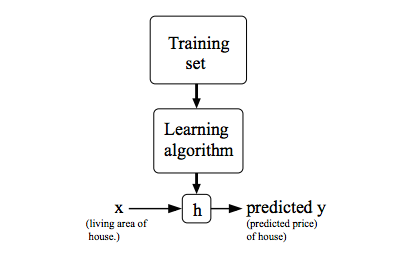
\includegraphics[ clip, scale=0.5]{img/process.png}
	\caption{ Process of machine learning }
	\label{fig.process }
\end{figure}
Another word, \textit{h} is a function that maps from x's to y's
When the target variable that we’re trying to predict is continuous, such as in our housing example, we call the learning problem a regression problem. When y can take on only a small number of discrete values (such as if, given the living area, we wanted to predict if a dwelling is a house or an apartment, say), we call it a classification problem. \\
\\
If \textit{h} is a function of one variable we called the model is \textbf{Univariate linear regression}
%-----------------------------------------------------------
% Third SECTION
%-----------------------------------------------------------
\subsection{Cost function}
Hypothesis: $h_{\theta}(x) = \theta_{0} + \theta_{1} \cdot x$

$\theta_{i}'s$: Parameters of the model

Cost function measures the accuracy of our hypothesis function. It is a function of parameters
\begin{equation*}
	J(\theta_0, \theta_1) = \dfrac {1}{2m} \displaystyle \sum _{i=1}^m \left ( \hat{y}^{(i)}- y^{(i)} \right)^2 = \dfrac {1}{2m} \displaystyle \sum _{i=1}^m \left (h_\theta (x^{(i)}) - y^{(i)} \right)^2
\end{equation*}

This function is otherwise called the "Squared error function", or "Mean squared error". The mean is halved ($\frac{1}{2}$) as a convenience for the computation of the gradient descent, as the derivative term of the square function will cancel out the $\frac{1}{2}$ term.
Now problem turns out of choosing value of $\theta_{0}$ and $\theta_1$. With each combination ($\theta_{0}$, $\theta_1$), we have a hypothesis (h) function.\\ \\
\textbf{Explain}:\\
	For each combination of ($\theta_{0}$, $\theta_1$), we have a value for hypothesis function. To find a closest $h(x)$ to actual data set means we have to find a combination of ($\theta_{0}$, $\theta_1$), such as $(h(x) - y)$ is minimum. \\ \\
	Lets consider whole training set, we have to find a combination of ($\theta_{0}$, $\theta_1$), such as the average of all difference: $\dfrac {1}{2m}\displaystyle \sum _{i=1}^m \left (h_\theta (x_{i}) - y_{i} \right)^2$ is minimum. Square the difference to cover the case hypothesis value is smaller than actual one. \\ \\
	
	If we call the difference above is cost function, the problem becomes find combination of ($\theta_{0}$, $\theta_1$) such as the cost function is smallest => Minimization problem
	
\subsubsection{Contour plot}
A contour plot is a graph that contains many contour lines. A contour line of a two variable function has a constant value at all points of the same line. An example of such a graph is the one to the right below.
\begin{figure}[h]
	\centering
	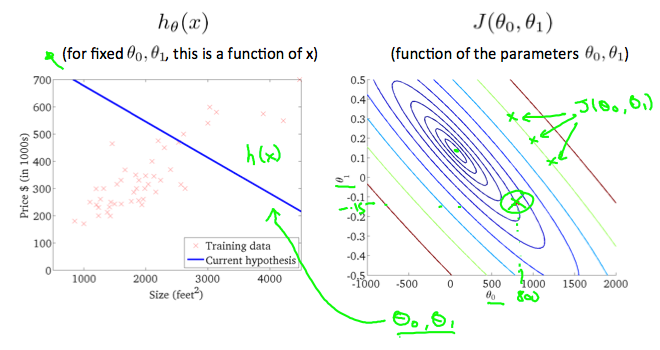
\includegraphics[ clip, scale=0.7]{img/contour_plot.png}
	\caption{ Contour plot }
	\label{fig.contour_plot}
\end{figure}
Taking any color and going along the 'circle', one would expect to get the same value of the cost function. For example, the three green points found on the green line above have the same value for $J(\theta_0,\theta_1)$ and as a result, they are found along the same line.

\newpage
\clearpage
\section{Algorithm gradient descent}
Here is the gradient descent algorithm:\\
\begin{equation}
\theta_j := \theta_j - \alpha \frac{\partial}{\partial \theta_j} J(\theta_0, \theta_1)
\end{equation}
where j=0,1 represents the feature index number.
\\
\\
Some important notes:
\begin{itemize}
	\item One should simultaneously update the parameters $\theta_1, \theta_2, ..., \theta_n$. Updating a specific parameter prior to calculating another one on the $j^{(th)}$ iteration would yield to a wrong implementation
	\item Taking the derivative (the tangential line to a function) of our cost function $J(\theta_0,\theta_1)$. The slope of the tangent is the derivative at that point and it will give us a direction to move towards
	\item The size of each step is determined by the parameter $\alpha$, which is called the learning rate. A smaller $\alpha$ would result in a smaller step and a larger $\alpha$ results in a larger step
	\item We make steps down the cost function in the direction with the steepest descent
	\item Depending on where one starts on the graph, one could end up at different points.
\end{itemize}